\section{Principaux algorithmes}
\subsection{Mouvements des pièces}
Pour le mouvement des pièces, nous avons choisi de le représenter comme
un arbre des positions. Un noeud et ses parents représentent tout le 
chemin pour arriver à la position au noeud. Voici un exemple :

\begin{figure}[H]
    \centering
    \begin{tabular}{|c|}
        \hline
        idx \\
        \hline
    \end{tabular} : case libre
    \begin{tabular}{|c|}
        \hline
        \cellcolor{gray}\color{white}idx \\
        \hline
    \end{tabular} : pion
    \begin{tabular}{|c|}
        \hline
        \cellcolor{green}\color{black}idx \\
        \hline
    \end{tabular} : pion à jouer
    \\
    \subfloat[Grille de jeu]{
        \begin{tabular}{|c|c|c|c|c|}
            \hline
            0                               & \cellcolor{gray}\color{white}1 & 2                              \\\hline
            \cellcolor{gray}\color{white}3  & 4                              & \cellcolor{gray}\color{white}5 \\\hline
            \cellcolor{green}\color{black}6 & \cellcolor{gray}\color{white}7 & 8                              \\\hline
        \end{tabular}
    }
    \\
    \raisebox{-0.5\height}{
        \subfloat[Arbre des mouvements possibles]{
            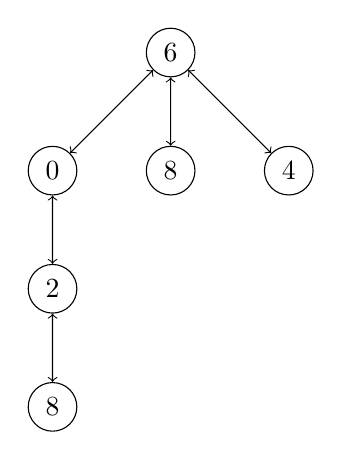
\begin{tikzpicture}[nodes={draw, circle}]
                \node {6}
                child {
                        node {0} edge from parent [<->]
                        child {
                                node {2} edge from parent [<->]
                                child {
                                        node {8} edge from parent [<->]
                                    };
                            };
                    }
                child {node {8} edge from parent [<->]}
                child {node {4} edge from parent [<->]};
            \end{tikzpicture}
        }
    }
    \hspace{1.5em}
    \raisebox{-0.5\height}{
        \subfloat[Ensemble des mouvements possibles]{
            \begin{tabular}{ ccccccccc }
                0 & 1 & 2 & 3 & 4 & 5 & 6 & 7 & 8 \\\hline
                \multicolumn{1}{|c|}{1}
                & \multicolumn{1}{|c|}{0} 
                & \multicolumn{1}{|c|}{1} 
                & \multicolumn{1}{|c|}{0} 
                & \multicolumn{1}{|c|}{1} 
                & \multicolumn{1}{|c|}{0} 
                & \multicolumn{1}{|c|}{0} 
                & \multicolumn{1}{|c|}{0} 
                & \multicolumn{1}{|c|}{1} 
                \\\hline
            \end{tabular}
        }
    }
    \caption{}
\end{figure}

Cet exemple nous montre 2 représentations des déplacements possibles pour
le pion à l'indice 6 sans compter les captures. L'ensemble à quelques avantages comparé à l'arbre.
Premièrement, pas besoin d'allocation dynamique, on peut juste faire un ensemble statiquement alloué
qui a la taille du monde. Ensuite, on a une complexité O(1) pour voir si on n'est pas déjà allé sur une case
lors de sauts multiples. L'implémentation en arbre, elle, doit être allouée dynamiquement,
et il y a une complexité O(h) pour voir si nous ne sommes pas déjà allé sur une case (grâce au double chaînage).
Mais, contrairement à l'implémentation avec un ensemble, nous pouvons savoir
exactement quel chemin a été emprunté pour aller à une position. Prenons les sauts
multiples pour arriver à la case 8. Dans le jeu des dames chinoises classique,
il y aurait une stratégie : est-ce que je prends le pion à la case 7, ou ceux aux cases 1 et 5 ?
Or, l'implémentation en ensemble ne permet pas de définir quel chemin nous avons emprunté.
Tandis qu'avec l'implémentation en arbre, il suffit de remonter l'arbre pour voir quel chemin nous avons emprunté.
Même si l'arbre complexifie le problème, il permet de rendre les mouvements bien plus génériques.


\subsection{Choix des meilleurs mouvements}
\subsubsection{BFS}
Pour pouvoir calculer les meilleurs mouvements, nous avons utilisé un Parcours en Largeur (Breadth First Search : BFS) sur le plateau. 
Premièrement on initialise la distance de toutes les cases avec une valeur maximale puis
le principe est de créer une file dans laquelle on ajoute toutes les positions de départ d'une couleur.
Ensuite tant que la file n'est pas vide, on récupère la position en tête, et pour chacun de ses voisins, 
si sa distance est inférieure on met à jour sa distance, qui est maintenant égale à la distance de notre position+1,
puis on l'enfile.
Ainsi chaque case se voit attribuer sa distance à la position de départ la plus proche pour une couleur. 
 
Cela nous permet d'avoir la distance d'une case donnée vers la position de départ d'une couleur avec une certaine relation. 
Ensuite il suffit de changer la relation et de relancer l'algorithme.
\subsubsection{Table de correspondance}

Ces distances sont enregistrées dans un tableau ce qui nous permet d'avoir une table de correspondance (\emph{lookup table}),
pour avoir en temps constant toutes les distances lors d'une partie vu que celle-ci est calculée lors de l'initialisation
du programme. Concernant la complexité en espace, elle réserve 
taille\_du\_monde * nombre\_de\_couleurs * nombre\_de\_relations * taille\_short\_int octets. Pour un jeu standard de configuration
 HEIGHT=4 WIDTH=5, avec 2 joueurs et 3 relations différentes, la taille allouée est de 240 octets, ce qui est correct.
Nous avons choisi d'utiliser des short int (2 octets) à la place des int (4 octets) pour réduire la taille totale allouée,
le seul inconvéniant que cela ajoute est que la distance maximale pouvant être enregistrée sans overflow est de \emph{65 535} mais cela
est largement suffisant pour nos utilisations.

Pour choisir le meilleur coup à jouer, on regarde parmi toutes les positions atteignables depuis 
notre case et on choisit celle dont la distance est la plus petite dans notre table de correspondance.

Nous avons opté pour une représentation de cette table par un tableau contigu en mémoire afin de favoriser le cache cpu
lors du BFS avec la localité spatiale et temporelle des accès mémoire. 

\begin{figure}[H]
\centering
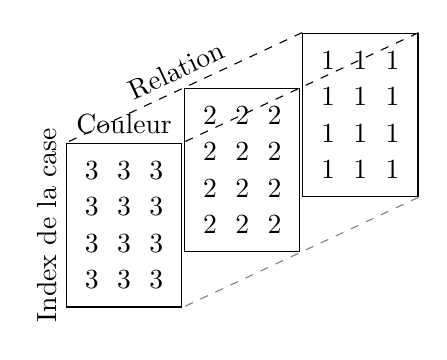
\begin{tikzpicture}
    \def\xs{1.5} %shift in x direction
    \def\ys{0.7} %shift in y direction
    \def\nm{3} % number of 2d matrices in the 3d matrix
    \foreach \x in {1,2,...,\nm}
    {
    
    \matrix [draw, % for the rectangle border
             fill=white, % so that it is not transparent
             ampersand replacement=\&] %see explanation
    (mm\x)%give the matrix a name
    at(-\x * \xs, -\x * \ys) %shift the matrix
    {
        \node {\x}; \& \node {\x}; \& \node {\x};\\
        \node {\x}; \& \node {\x}; \& \node {\x};\\
        \node {\x}; \& \node {\x}; \& \node {\x};\\
        \node {\x}; \& \node {\x}; \& \node {\x};\\
    };
    }
    
    \draw [dashed,black](mm1.north west) -- node[sloped,above] {Relation} (mm\nm.north west);
    \draw [dashed,black](mm1.north east) -- (mm\nm.north east);
    \draw [dashed,gray](mm1.south east) -- (mm\nm.south east);

    \node [rotate=90][above] at (mm3.west) {Index de la case};
    \node [above] at (mm3.north) {Couleur};
    
\end{tikzpicture}
\caption{Représentation de la table de correspondance}
\end{figure}


